\documentclass[a4paper,11p]{memoir}

\pdfoutput=1

\newlength{\figwidth}
% FINAL
%\setlength{\figwidth}{88mm}
% DRAFT
\setlength{\figwidth}{0.65\textwidth}


\usepackage{color}
\definecolor{links}{rgb}{0.7,0,0}   % red
\definecolor{urls}{rgb}{0,0,0.8}    % blue
\definecolor{cites}{rgb}{0,0,0.8}   % blue

\usepackage[colorlinks,hyperindex,linkcolor=links,citecolor=cites,urlcolor=urls]{hyperref} % generates colored links in pdf file
 
%---------------------------------------------------------
% styles and other macros
\usepackage[nosort]{cite}        
\usepackage{url} 
\usepackage[intlimits]{amsmath}
\usepackage{bbm}
\usepackage{graphicx}
\usepackage{paralist}
\usepackage{verbatim}
\usepackage[stretch=16,shrink=16,step=4]{microtype}
% \usepackage{vmr-symbols-vecbold}
% \usepackage{standard-macros}


\def\matn{\mathcal{N}}

%*******************************************************************************
%!TEX encoding =  

\begin{document}


\title{SPeCTrE\\
Short Packet Communication Toolbox for Wireless Engineers\\[1cm]
Version 0.0}

\maketitle

\begin{abstract}
  
\end{abstract}
\newpage
\tableofcontents

\newpage
%%%%%%%%%%%%%%%%%%%%%%%%%
\chapter{Motivation}
%%%%%%%%%%%%%%%%%%%%%%%%%
\chapter{AWGN channel}


General info:
\begin{itemize}
\item Maintainer: Y. Polyanskiy \url{<yp@mit.edu>}

\item Main references: \cite{PPV08,PPV10eneff}

\item Example: See Fig.~\ref{fig:awgn_example} 

\item Channel model:
	$$ Y_j = X_j + Z_j, \quad j=1,\ldots,n $$
	Noise: $Z_j \sim \matn(0,1)$ iid.\\
	Power constraints: Each codeword $x^n$ satisfies
			$$ \sum_{j=1}^n |x_j|^2 \le n P $$

\item Common input/output arguments:
\begin{enumerate}
\item \verb|P| -- input argument; parameter of the power constraint (so $P=10$ is $SNR=10~dB$).
\item \verb|epsil| -- block probability of block error.
\item \verb|lm| or \verb|Lms| -- output argument; $\log_2 M$, log-size of codebook (base-2 information units). 
\item \verb|n| -- input argument; blocklength.\\
		For slow functions that do not support vectorized arguments.
\item \verb|Ns| -- input argument; vector of blocklengths.
\end{enumerate}
\end{itemize}


\begin{figure}
\begin{verbatim}
	> plot_v3(10, 0.001, 1, 100:20:1000)
\end{verbatim}
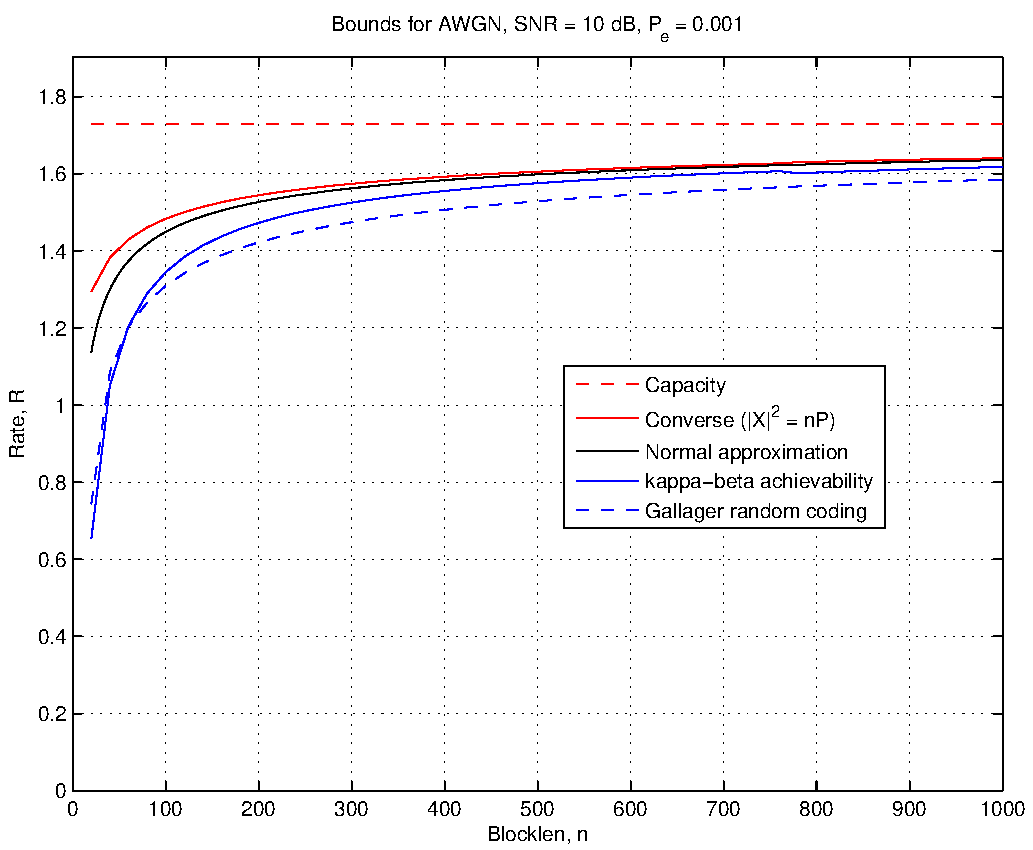
\includegraphics[height=5cm]{plots/awgn_plot3_ex.pdf}
\caption{Code and resulting picture for AWGN bounds}\label{fig:awgn_example}
\end{figure}


\section{Summary plot: \texttt{plot\_v3()}}

Definition:
\begin{verbatim}
	function [Ns lb ub feinst gal wlfz] = plot_v3(P, epsil)
\end{verbatim}

This function plots various bounds on the same figure. See Fig.~\ref{fig:awgn_example}.


\section{Achievability: \texttt{shannon\_ach2()}}

Definition:
\begin{verbatim}
	function lm = shannon_ach2(n, epsil, P)
\end{verbatim}

Function computes Shannon's cone-packing achievability bound, see~\cite[(41)]{PPV08}.

\section{Achievability: \texttt{kappabeta\_ach()}}
Format:
\begin{verbatim}
	function Lms = kappabeta_ach(Ns, epsil, P, hack)
\end{verbatim}

This computes the $\kappa\beta$ achievability bound, see left-hand inequality in~\cite[(218)]{PPV08}. If $hack\neq 0$, then we
use asymptotic approximation for $\kappa$. This increases the speed dramatically and is very precise already at $n=10$,
see~\cite[(217)]{PPV08}. If $hack$ is not set, it defaults to $1$.

\section{Achievability: \texttt{gallager\_ach()}}
Format:
\begin{verbatim}
	function lm = gallager_ach(n, epsil, P)
\end{verbatim}

Computes Gallager's achievability bound, see~\cite[(44)]{PPV08}.

\section{Converse: \texttt{converse()}}
Format:
\begin{verbatim}
	function Lms = converse(Ns, epsil, P)
\end{verbatim}

This computes the meta-converse lower bound with $Q_{Y^n} = \matn(0, 1+P)^n$, see right-hand inequality in~\cite[(218)]{PPV08}. 


\section{Normal approximation: \texttt{normapx\_awgn(), normapx\_biawgn()}}

Format:
\begin{verbatim}
	function Lms = normapx_awgn(Ns, epsil, P);
\end{verbatim}

Fast and frequently very precise approximation to both achievability and converse:
	$$ \log M \approx n C - \sqrt{nV} Q^{-1}(\epsilon) + {1\over2} \log n $$


\section{Code database: \texttt{plot\_universe()}}

Code in \verb|universe/plot_universe()| compiles a comparative plot of normalized rate for different codes.
See~\cite[Section IV.D]{PPV08}.


\section{Energy-per-bit bounds}

\textbf{TODO}.

%%%%%%%%%%%%%%%%%%%%%%%%%
%\chapter{Fading channels}
%%%%%%%%%%%%%%%%%%%%%%%%%%%%
\bibliographystyle{IEEEtran}
\bibliography{IEEEabrv,refs}
\end{document}

